\documentclass[12pt,a4paper]{scrartcl}
\usepackage[latin1]{inputenc}
\usepackage{amsmath}
\usepackage{amsfonts}
\usepackage{amssymb}
\usepackage{graphicx}
\graphicspath{{images/}}
\usepackage{wrapfig}
\usepackage{fancyhdr}
\usepackage{lastpage}

\date{}
\linespread{1.5}
\pagestyle{fancy}
\fancyhf{}
\fancyhead[LO]{\today}
\fancyhead[CO]{[Filthy Cell-Culture Dish]}
\fancyfoot[R]{Page \thepage\ of \pageref{LastPage}}
\renewcommand{\headrulewidth}{0pt}% disable the underline of the header part


%\setheadsepline{.4pt}
%\setfootsepline{.4pt}
\usepackage[bookmarks=true]{hyperref}
\usepackage{bookmark}
\begin{document}
\begin{center}
\thispagestyle{empty}
\vfill
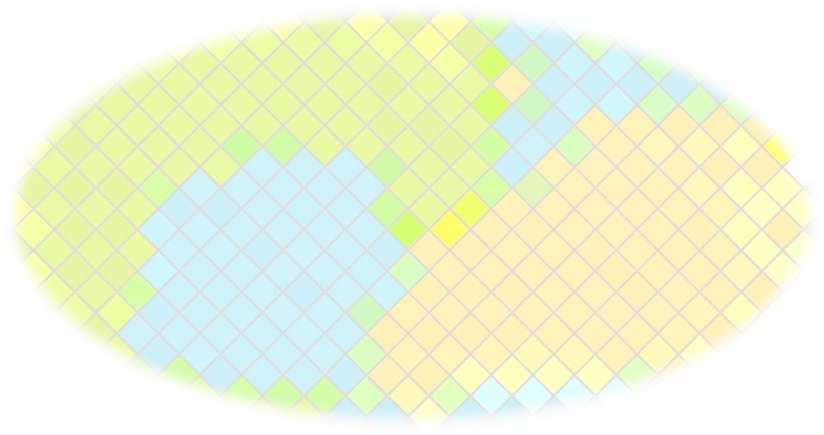
\includegraphics[scale=1]{title2}
\vfill
\huge
	\textbf{Filthy Cell-Culture Dish\\
	User Manuel\\}
\vfill
\large
	(c) YYL Team\\
	Based on Version 1.0.0
\vfill
\end{center}

\clearpage

\large
\textbf{Project Team}
\begin{itemize}
	\item Boyuan Yuan
	\begin{flushright}
		Developer\\
		Storyteller\\
		Graphic Designer\\
		Artwork\\
	\end{flushright}
	
	\item Chunchuan Lv
	\begin{flushright}	
		Developer\\
		Tester\\
		Graphic\\
		Debugger\\
	\end{flushright}
	
	\item Yue Yu
	\begin{flushright}
		Developer\\
		Documentation\\
		Graphic Designer\\
		Artwork\\
	\end{flushright}
\end{itemize}
\clearpage

\large
\textbf{Recommended Requirements}
\begin{list}{}{}
	\item \textbf{CPU:} 2.0GHz i3 Dual Core or equivalent
	\item \textbf{RAM:} 1 GB
	\item \textbf{OS:} Windows 7 or later, Mac OS X 10.8+, GNU/Linux kernel 2.6.18 or later
	\item \textbf{Video Card:} Yes
	\item \textbf{Sound Card:} Yes
	\item \textbf{Free Disk Space:} 500 MB
\end{list}
\clearpage
% Inhaltsverzeichnis	
\pdfbookmark[1]{\contentsname}{toc}\tableofcontents
\clearpage

\section{Introduction to The Game}

This game is a strategy game. Each player creates and evolves a kind of bacteria in an effort to populate the span of a culture dish in a biological laboratory. The game uses a population model with a complex and realistic set of variables and rules to simulate the evolution and competition of the bacteria. Player will be in charge with macro manage: the evolutionary path of his/her species and micro manage: exploration of the small world. The purpose of the game is to take the species into prosperity.

\section{Game Terms}

\subsection{Cell}

The world in the game is represented by consecutive cells. Individual cell has properties of current population of species and its' environmental limit. There will be additional statistics available for player for decision making.

\subsection{Turn}

Players take turns when playing. During each turn, a player can choose a cell to explore, select a trait to upgrade (if available) and check the status of the current game session. For demonstration, all the players will play on the same host.

\subsection{Explore}

During every turn, each player can choose a cell to explore by clicking that cell and a population advantage for that player's specie will be added to the cell. Players will be challenged to make decisions under an environment of uncertainty. The exploration element allows player treat the game like GO.

\subsection{Traits}

New traits will be obtained as game progress. At the end of each turn, if enough mutation is culminated, current selected trait will be advanced into next stage. The required mutation will be determined by whether this level of trait is obtained by other species (if it does, there is a discount) and current level of the trait. 

The traits in this game is consisted of five main categories: Growth Trait, Explore Trait, Attack Trait, Defense Trait and Ultimate Trait.


\begin{itemize}
	\item Growth Trait
	\begin{itemize}
		\item Expanding pace of species' population in a cell
	\end{itemize}
	\item Exploring Trait
	\begin{itemize}
		\item Population advantage of exploration act
		\item Threshold for expanding to neighbor cells
	\end{itemize}
	\item Attacking Trait
	\begin{itemize}
		\item Positive factor for your specie during the battle among species
	\end{itemize}
	\item Defensive Trait
	\begin{itemize}
		\item Negative factor for other species during the battle among species
	\end{itemize}
	\item Ultimate Trait
	\begin{itemize}
		\item The very only approach to win the game with a special trait. This trait will enable the specie to fly out of the culture dish and earn victory
	\end{itemize}
\end{itemize}

\section{Download the Game}

\section{Start the Game}
This game is build by Unity and no installation procedure is needed before running the game. Just unzip the downloaded game package and double click the main program, the game will run.

\subsection{Screen Resolution Choice}

$1024\times640$ and other 16:9 screens with higher resolution are suggested.

\subsection{Main Menu}
The first scene will be shown is the main menu of the game. In this menu, players can start the game, review credits and turn on or off the sound effect.
\begin{figure}[h] 
	\centering
	
\includegraphics[scale=0.2]{start1}
	\caption{Main menu of the game}
\end{figure}

\subsection{Difficulty Level}
The following scene will allow the user to choose a difficulty level for the game. In this demo version, the difficulty of all three levels will be the same.
\begin{figure}[h] 
	\centering
	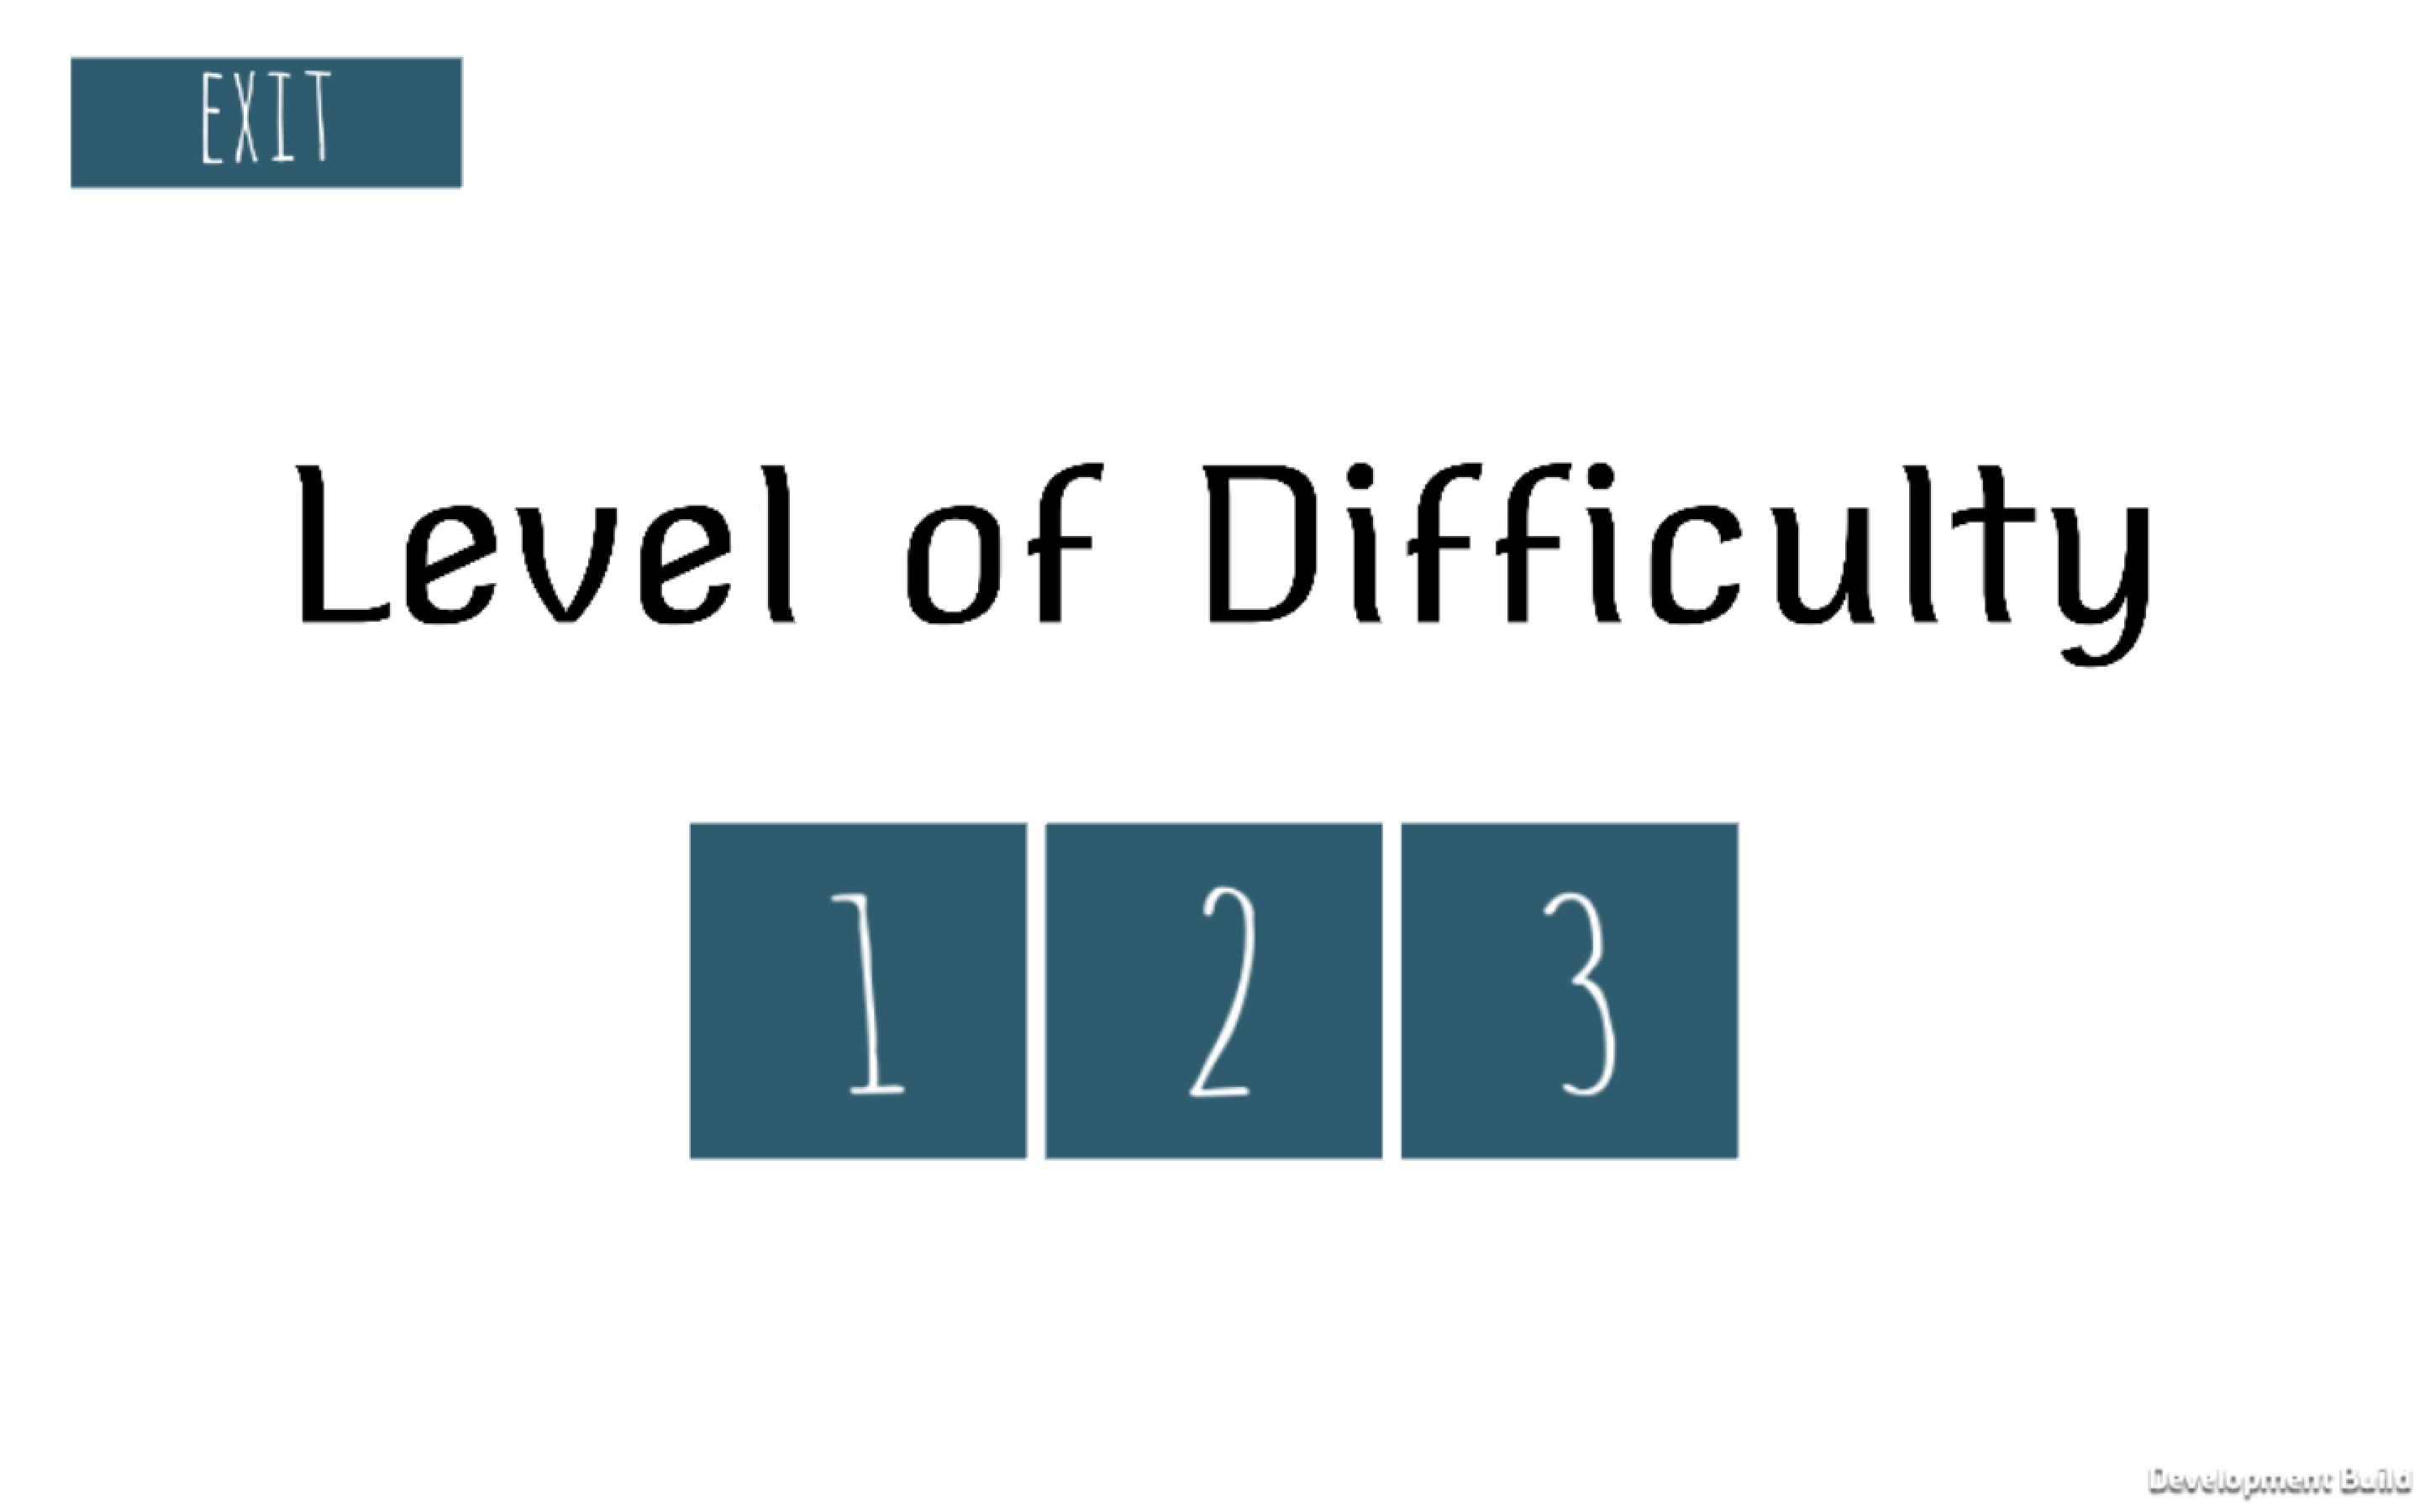
\includegraphics[scale=0.2]{start2}
	\caption{Main menu of the game}
\end{figure}

\subsection{Game Options}
The next menu will allow players to configure several essential game settings in the way they like, such as the number of players, the maximum turns allowed, the width of the map and the height of the map. It should be noticed that, the last three parameters should be equal or larger than 10.

\begin{figure}[h] 
	\centering
	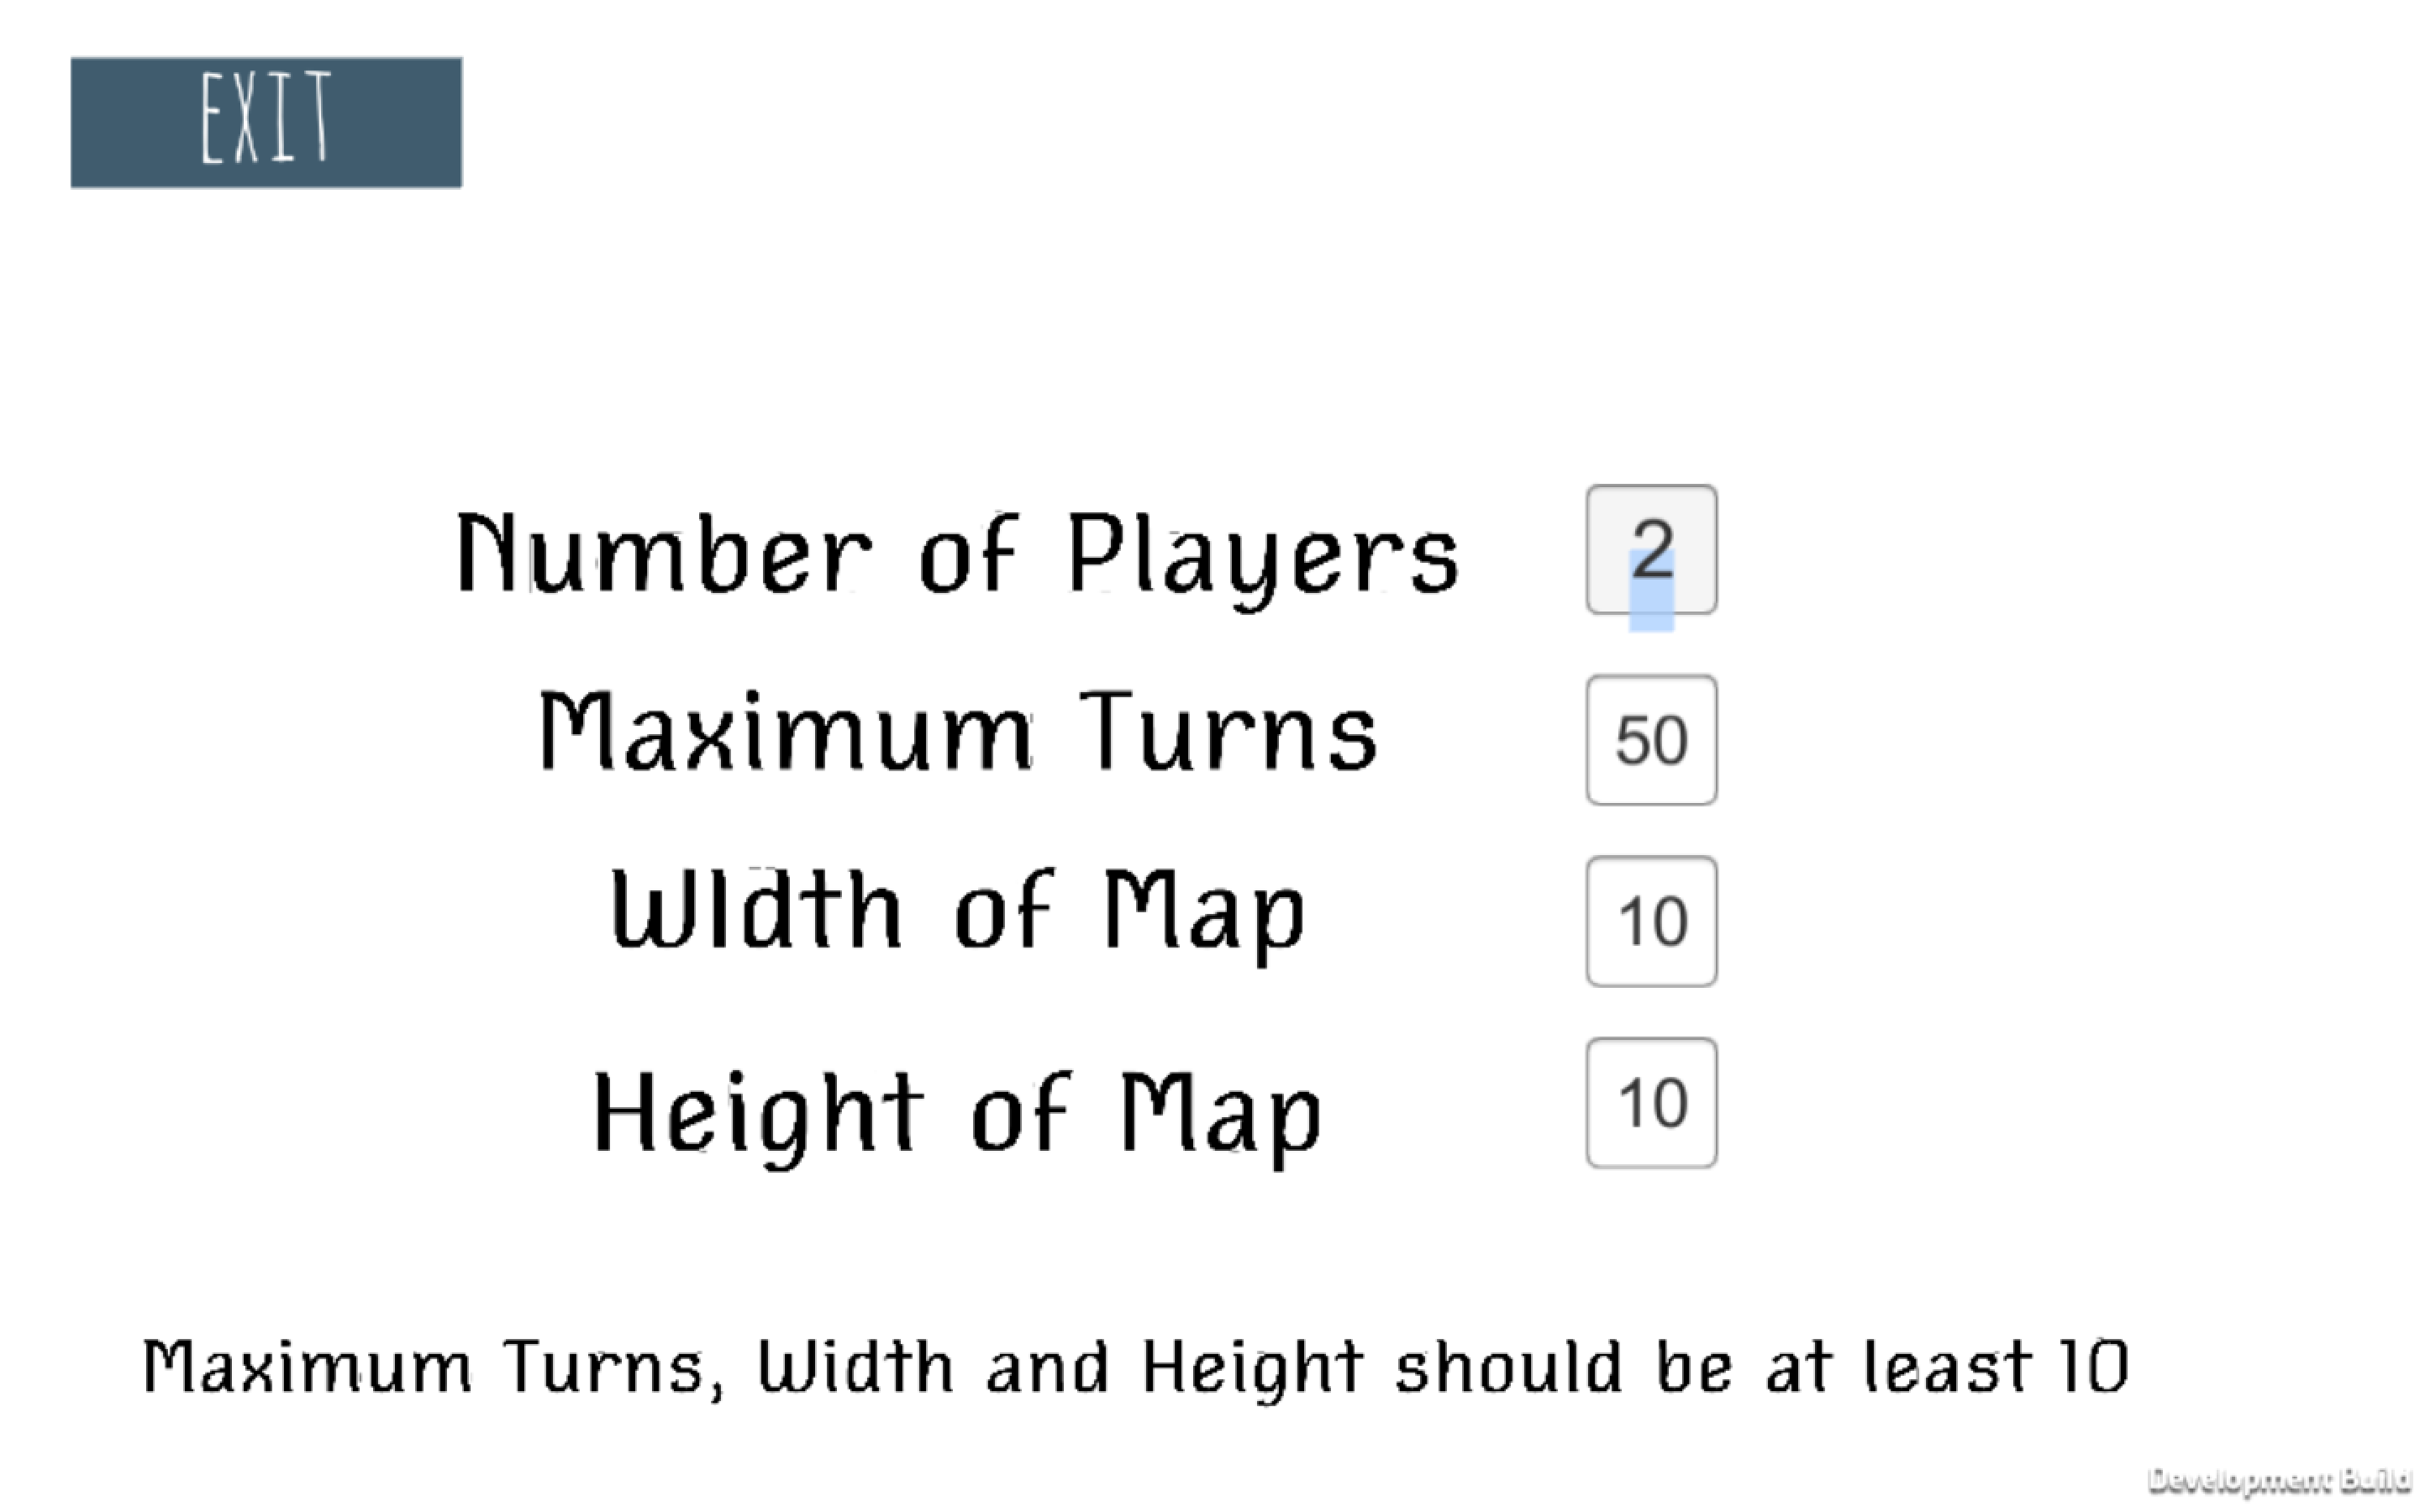
\includegraphics[scale=0.2]{start3}
	\caption{Main menu of the game}
\end{figure}

Press [Enter], after finishing the configuration, to start the game.
\section{Exit the Game}
During the game session, players can press [esc] at any time to exit the game. All the user data of current session will be lost.

\section{Victory Conditions}
There are three conditions for victory. They are domination victory, time victory, and evolution victory.
\begin{itemize}
	\item Domination Victory
	\newline A species has over 50\% of maximum population
	\item Time Victory 
	\newline Species with most population wins if game does not end within specified maximum turns
	\item Evolution Victory
	\newline A trait of moving out of cells is developed to ultimate level.
\end{itemize}

\end{document}